% !TEX root = ../main.tex
% Бүлэг 2

\chapter{Платформын шинжилгээ ба шаардлага}
\label{Chapter2}

\section{Одоогийн нөхцөл байдлын шинжилгээ}
Удиртгалд дурдсанчлан Монголын загварын мэдээлэл олон сувгаар тархсан байдалтай. Энэ хэсэгт тухайн нөхцөл байдлыг сувгийн төрөл, контентын шинж, хэрэглэгчийн хайлтын боломж гэсэн чиглэлээр нарийвчлан шинжилнэ. Загварын брэндүүд шинэ коллекц, бүтээгдэхүүн, эвентийн мэдээллээ ихэвчлэн social media, өөрийн веб хуудас, e-commerce хуудас, lifestyle медиа, эвентийн зарын хэлбэрээр нийтэлдэг. Сувгийн тархалтын улмаас хэрэглэгч нэг дизайнерын collection, lookbook, нийтлэл, designer profile, trend content-ийг нэг дороос хайж үзэхэд хүндрэлтэй болдог.

Сувгуудын нийтлэлийн хэлбэр, хадгалалт, хайлтын боломжийг шинжлэхэд дараах нийтлэг асуудал илэрнэ. Нэгдүгээрт, fashion content-д зориулсан тусдаа мэдээллийн бүтэц сул байна. Хоёрдугаарт, өмнөх collection, lookbook, event, нийтлэлийн archive тогтвортой хадгалагдахгүй байх тохиолдол бий. Гуравдугаарт, хайлт, category, tag, designer, season, material зэрэг шүүлтүүрийн боломж хангалтгүй. Дөрөвдүгээрт, Монголын загварын контентыг editorial маягийн сэтгүүлийн хэлбэрээр, зурагт өгүүлэмжтэйгээр үзүүлэх digital magazine туршлага хомс байна.

Зураг \ref{fig:ch2-current-content-distribution}-т одоогийн загварын контентын тархалтын ерөнхий байдлыг харуулав. Social media, брэндийн веб, lifestyle медиа, e-commerce, fashion event-ийн мэдээлэл тус тусдаа оршиж байгаа нь хэрэглэгчийн хайлт болон судалгааны ажлыг удаашруулдаг.
\begin{figure}[htbp]
  \centering
  \resizebox{0.92\textwidth}{!}{\begin{tikzpicture}[x=1cm,y=1cm,>=stealth,thick]
  \tikzstyle{source}=[draw, rounded corners=5pt, minimum width=3.8cm, minimum height=0.85cm,
    text width=3.35cm, align=center, font=\scriptsize]
  \tikzstyle{centerbox}=[draw, rounded corners=6pt, minimum width=4.4cm, minimum height=1.05cm,
    text width=3.95cm, align=center, font=\scriptsize\bfseries]
  \tikzstyle{note}=[draw, rounded corners=5pt, minimum width=4.2cm, minimum height=0.85cm,
    text width=3.8cm, align=center, font=\scriptsize]

  \node[source, fill=blue!8] (social) at (0,4.8) {Social media\\пост, story, reel};
  \node[source, fill=green!8] (brand) at (5.2,4.8) {Брэндийн веб\\product/story};
  \node[source, fill=yellow!12] (media) at (10.4,4.8) {Lifestyle медиа\\нийтлэл};
  \node[source, fill=orange!10] (shop) at (2.6,2.7) {E-commerce\\бүтээгдэхүүн};
  \node[source, fill=purple!8] (event) at (7.8,2.7) {Fashion event\\зар, recap};

  \node[centerbox, fill=gray!12] (user) at (5.2,0.8) {Хэрэглэгч\\загварын мэдээлэл хайна};
  \node[note, fill=red!6] (problem) at (5.2,-1.2) {Мэдээлэл салангид, archive сул,\\хайлт ба ангилал хангалтгүй};
  \node[note, fill=cyan!8] (platform) at (5.2,-3.1) {Нэгдсэн fashion magazine\\ба digital archive платформын хэрэгцээ};

  \draw[->] (social) -- (user);
  \draw[->] (brand) -- (user);
  \draw[->] (media) -- (user);
  \draw[->] (shop) -- (user);
  \draw[->] (event) -- (user);
  \draw[->] (user) -- (problem);
  \draw[->] (problem) -- (platform);
\end{tikzpicture}
}
  \caption[Одоогийн загварын контентын тархалт]{Одоогийн загварын контентын тархалтын ерөнхий байдал}
  \label{fig:ch2-current-content-distribution}
\end{figure}

Хүснэгт \ref{tab:current-web-context} нь одоогийн цахим орчны давуу болон сул талыг нэгтгэн харуулна. Энэ шинжилгээ нь нэгдүгээр бүлэгт авч үзсэн Vogue Runway, Tagwalk, Google Arts \& Culture Fashion, CFDA Runway360 зэрэг төстэй платформын судалгаатай холбогдоно. Тэдгээр платформуудын нийтлэг давуу тал нь контентыг category, designer, collection, season, archive хэлбэрээр системтэй хадгалж, хэрэглэгчид editorial болон visual discovery туршлага өгдөг явдал юм.

\begin{longtable}{|L{0.22\textwidth}|L{0.31\textwidth}|L{0.33\textwidth}|}
  \hline
  \textbf{Суваг} & \textbf{Давуу тал} & \textbf{Хязгаарлалт} \\ \hline
  Social media & Шуурхай, зурагт пост хурдан түгдэг & Archive, хайлт, category сул; мэдээлэл timeline-д алдагдана \\ \hline
  Брэндийн веб хуудас & Брэнд өөрийн бүтээгдэхүүн, collection-оо албан ёсоор танилцуулна & Олон брэндийн мэдээлэл нэг дор төвлөрөхгүй \\ \hline
  Lifestyle медиа & Загварын нийтлэл, ярилцлага, trend content гаргадаг & Collection/lookbook metadata тогтмол бүтэцтэй хадгалагдахгүй \\ \hline
  E-commerce платформ & Бүтээгдэхүүн, үнэ, худалдан авалтын мэдээлэл тодорхой & Editorial story, дизайнерын түүх, архивын утга сул \\ \hline
  Fashion event мэдээлэл & Шинэ эвент, runway, preview-ийн мэдээлэл хүргэнэ & Event дууссаны дараа системтэй archive үүсэхгүй байх магадлалтай \\ \hline
  \caption{Одоогийн веб орчны давуу болон сул тал}
  \label{tab:current-web-context}\\
\end{longtable}

\section{Платформын хамрах хүрээ}
Удиртгалд тодорхойлсон зорилгод үндэслэн энэ хэсэгт платформын хамрах функциональ хүрээ, хэрэглэгчийн хэсгүүд, техникийн хил хязгаарыг нарийвчлан тогтоов. Платформ нь blog хэлбэрийн нэг чиглэлийн нийтлэл бус, fashion magazine болон digital archive-ийн хоёр шинжийг нэгтгэсэн веб систем юм.

Хэрэглэгчийн хэсэгт нүүр хуудас, archive, editorial, designers, collection detail, article detail, search overlay, profile зэрэг дэлгэц орно. Админ хэсэгт login, dashboard, нийтлэл удирдах, collection удирдах, designer удирдах, media asset удирдах, хэрэглэгчийн эрх зохицуулах боломж орно. Техникийн хүрээнд Next.js/React frontend, Next.js API route, CouchDB content repository, Supabase authentication/profile/bookmark/RAG layer, Tailwind CSS styling, TypeScript domain type ашиглагдана.

Хүснэгт \ref{tab:scope-in-out}-д платформын хамрах болон хамрахгүй хүрээг харуулав. Хамрахгүй хүрээг тодорхойлох нь дипломын ажлын бодит хэмжээг хэт тэлэхээс сэргийлнэ.

\begin{longtable}{|L{0.20\textwidth}|L{0.36\textwidth}|L{0.30\textwidth}|}
  \hline
  \textbf{Төрөл} & \textbf{Хүрээ} & \textbf{Тайлбар} \\ \hline
  Хамрах & Хэрэглэгчийн public хэсэг & Нүүр, нийтлэл, archive, designer, collection, хайлт \\ \hline
  Хамрах & Админ хэсэг & Dashboard, article/collection/designer/asset management \\ \hline
  Хамрах & Category/tag бүтэц & Нийтлэл болон archive контентыг ангилах, шүүх \\ \hline
  Хамрах & Authentication ба authorization & Supabase session, admin/editor/viewer role шалгалт \\ \hline
  Хамрах & API холболт & Public content API, protected admin API, chat API \\ \hline
  Хамрах & Өгөгдлийн сан & CouchDB document store, Supabase profile/bookmark/RAG өгөгдөл \\ \hline
  Хамрах & Visual content & Thumbnail, cover image, look image, media asset \\ \hline
  Хамрахгүй & Payment систем & Худалдан авалт, төлбөрийн урсгал дипломын хүрээнд орохгүй \\ \hline
  Хамрахгүй & Бүрэн social network & Like/comment/feed/message зэрэг том social module хийхгүй \\ \hline
  Хамрахгүй & Native mobile app & Responsive web хэрэгжинэ, тусдаа iOS/Android app хийхгүй \\ \hline
  Хамрахгүй & Том хэмжээний production optimization & CDN, multi-region scaling, enterprise traffic tuning хийхгүй \\ \hline
  \caption{Платформын хамрах ба хамрахгүй хүрээ}
  \label{tab:scope-in-out}\\
\end{longtable}

\section{Хэрэглэгчийн шаардлагын шинжилгээ}
Платформын үндсэн хэрэглэгчийг зочин хэрэглэгч, бүртгэлтэй хэрэглэгч, админ/редактор гэж ангилна. Зочин хэрэглэгч login хийхгүйгээр нийтлэл унших, category сонгох, archive үзэх, хайлт хийх боломжтой байна. Бүртгэлтэй хэрэглэгч public боломж дээр нэмээд profile, bookmark зэрэг хувийн үйлдэл ашиглана. Админ/редактор нь нийтлэл, зураг, collection, designer, category/tag, хэрэглэгчийн эрхийг удирдах зорилготой.

Хэрэглэгчийн шаардлагыг тодорхойлохдоо хэрэглэгч бүрийн зорилго, хийх үйлдэл, хэрэгтэй мэдээлэл, хязгаарлалтыг авч үзэв. Зочин хэрэглэгчийн гол шаардлага нь navigation ойлгомжтой, хайлт хурдан, зураг болон текстийн layout эвтэйхэн байх явдал юм. Админы гол шаардлага нь хамгаалалттай нэвтрэх, form validation, зураг оруулах, draft/review/published төлөв удирдах, алдаа гарсан үед ойлгомжтой мэдээлэл авах явдал юм.

\begin{longtable}{|L{0.16\textwidth}|L{0.22\textwidth}|L{0.26\textwidth}|L{0.18\textwidth}|}
  \hline
  \textbf{Хэрэглэгч} & \textbf{Зорилго} & \textbf{Үндсэн үйлдэл} & \textbf{Шаардлага} \\ \hline
  Зочин хэрэглэгч & Монголын загварын нийтлэл, archive үзэх & Нийтлэл унших, category сонгох, хайлт хийх, collection үзэх & Хялбар navigation, responsive UI \\ \hline
  Бүртгэлтэй хэрэглэгч & Сонирхсон контентоо хадгалах & Login хийх, bookmark хийх, profile үзэх & Session найдвартай, хадгалалт тодорхой \\ \hline
  Редактор & Контент бэлтгэх, засварлах & Нийтлэл нэмэх, зураг upload хийх, draft/review төлөв сонгох & Form validation, media upload, protected route \\ \hline
  Админ & Платформын контент ба эрх удирдах & Нийтлэх, устгах, role өөрчлөх, invite илгээх & Role-based access, audit-friendly workflow \\ \hline
  \caption{Хэрэглэгчийн төрөл ба шаардлага}
  \label{tab:user-types-requirements}\\
\end{longtable}

\section{Функциональ шаардлага}
Функциональ шаардлага нь платформ ямар үйлдэл хийж чаддаг байх ёстойг тодорхойлно. Энэ платформын хувьд public унших урсгал, хайлт/ангилал, archive, authentication, admin CMS, API, media upload, AI туслах гэсэн бүлгүүдээр шаардлагыг тодорхойлов.

{\small
\begin{longtable}{|L{0.07\textwidth}|L{0.24\textwidth}|L{0.35\textwidth}|L{0.16\textwidth}|}
  \hline
  \textbf{Код} & \textbf{Шаардлага} & \textbf{Тайлбар} & \textbf{Хэрэглэгч} \\ \hline
  FR-01 & Нүүр хуудас үзэх & Хэрэглэгч платформын brand identity, онцлох collection, editorial entry үзнэ & Зочин, хэрэглэгч \\ \hline
  FR-02 & Нийтлэл жагсаалтаар харах & Published нийтлэлүүд category болон огноогоор харагдана & Зочин, хэрэглэгч \\ \hline
  FR-03 & Нийтлэлийн дэлгэрэнгүй үзэх & Нийтлэлийн гарчиг, зураг, body, tag, холбоотой контент харагдана & Зочин, хэрэглэгч \\ \hline
  FR-04 & Category/tag-аар шүүх & Хэрэглэгч нийтлэл болон archive контентыг ангиллаар шүүнэ & Зочин, хэрэглэгч \\ \hline
  FR-05 & Хайлт хийх & Search overlay нь article, collection, designer result харуулна & Бүх хэрэглэгч \\ \hline
  FR-06 & Archive үзэх & Collection, season, year, designer, look image, material үзэх боломжтой байна & Зочин, хэрэглэгч \\ \hline
  FR-07 & Designer profile үзэх & Дизайнерын bio, brand, холбоотой collection харагдана & Зочин, хэрэглэгч \\ \hline
  FR-08 & Bookmark хийх & Нэвтэрсэн хэрэглэгч сонирхсон контентоо хадгална & Бүртгэлтэй хэрэглэгч \\ \hline
  FR-09 & Админ нэвтрэх & Staff хэрэглэгч login хийж protected admin хэсэгт орно & Админ, редактор \\ \hline
  FR-10 & Нийтлэл нэмэх & Админ/редактор title, subtitle, body, category, tag, image оруулж нийтлэл үүсгэнэ & Админ, редактор \\ \hline
  FR-11 & Нийтлэл засах & Одоо байгаа нийтлэлийн мэдээлэл, зураг, төлөв шинэчлэгдэнэ & Админ, редактор \\ \hline
  FR-12 & Нийтлэл устгах & Шаардлагагүй нийтлэл баталгаажуулалтын дараа устгагдана & Админ, редактор \\ \hline
  FR-13 & Зураг оруулах & Cover image, look image, profile image media asset хэлбэрээр хадгалагдана & Админ, редактор \\ \hline
  FR-14 & Category/tag удирдах & Контент ангилахад ашиглах metadata сонгох, хадгалах боломжтой байна & Админ, редактор \\ \hline
  FR-15 & Authorization шалгах & Admin API бүр user session болон role шалгана & Систем \\ \hline
  FR-16 & API-аар өгөгдөл авах/илгээх & Frontend public/admin API route-уудаар өгөгдөл солилцоно & Систем \\ \hline
  FR-17 & AI туслах ашиглах & Chat API live archive болон RAG context ашиглан лавлагаа өгнө & Бүртгэлтэй хэрэглэгч \\ \hline
  \caption{Функциональ шаардлагын жагсаалт}
  \label{tab:functional-requirements-ch2}\\
\end{longtable}
}

\section{Функциональ бус шаардлага}
Функциональ бус шаардлага нь платформын чанарын түвшинг тодорхойлно. Загварын сэтгүүлийн платформ нь зурагт контент ихтэй, public болон admin хэрэглэгчийн урсгал зэрэгцээ ажилладаг тул гүйцэтгэл, responsive design, security, usability, maintainability онцгой чухал.

\begin{longtable}{|L{0.10\textwidth}|L{0.24\textwidth}|L{0.48\textwidth}|}
  \hline
  \textbf{Код} & \textbf{Шаардлага} & \textbf{Тайлбар} \\ \hline
  NFR-01 & Гүйцэтгэл & Хуудас хурдан ачаалж, зураг боломжийн хэмжээтэй, хайлт debounce/ranking ашиглан саадгүй ажиллана \\ \hline
  NFR-02 & Хэрэглэхэд хялбар байдал & Navigation ойлгомжтой, нийтлэл унших болон archive хайх урсгал богино байна \\ \hline
  NFR-03 & Responsive design & Desktop, tablet, mobile дэлгэц дээр layout, text, button, image давхцахгүй байна \\ \hline
  NFR-04 & Аюулгүй байдал & Admin route, admin API, role update, invite зэрэг үйлдэл session болон role шалгалтаар хамгаалагдана \\ \hline
  NFR-05 & Найдвартай ажиллагаа & API алдаа, хоосон search result, upload алдаа гарвал хэрэглэгчид ойлгомжтой мэдэгдэнэ \\ \hline
  NFR-06 & Өргөтгөх боломж & Шинэ category, designer profile, event calendar, semantic search зэрэг module нэмэхэд бүтэц саад болохгүй \\ \hline
  NFR-07 & Засварлахад хялбар байдал & Component-based UI, repository layer, typed domain model ашиглан кодын хамаарлыг багасгана \\ \hline
  NFR-08 & Контентын зохион байгуулалт & Article, category, tag, image, collection, designer хоорондын холбоо ойлгомжтой байна \\ \hline
  NFR-09 & Нууцлал & API key, database credential зэрэг sensitive data client bundle-д ил гарахгүй, environment variable ашиглана \\ \hline
  NFR-10 & AI хариултын найдвартай байдал & Context байхгүй үед зохиомол баримт өгөхгүй, fallback тайлбар харуулна \\ \hline
  \caption{Функциональ бус шаардлага}
  \label{tab:nonfunctional-requirements-ch2}\\
\end{longtable}

\section{Юзкейс диаграмм}
Use case диаграмм нь платформд оролцох actor болон тэдгээрийн хийж болох үйлдлийг ерөнхийлөн харуулна. Энэ платформд зочин хэрэглэгч, бүртгэлтэй хэрэглэгч, редактор, админ гэсэн actor оролцоно. Зочин хэрэглэгч public контент үзэж, search/archive ашиглана. Бүртгэлтэй хэрэглэгч bookmark болон profile ашиглана. Редактор нийтлэл, collection, designer, asset мэдээлэл бэлтгэнэ. Админ эдгээр үйлдэл дээр нэмээд user role, invite, нийтлэх эрхийг удирдана.

\begin{figure}[htbp]
  \centering
  \resizebox{0.96\textwidth}{!}{\begin{tikzpicture}[x=1cm,y=1cm,>=stealth]

  % --- Styles ---
  \tikzset{
    actorlabel/.style={font=\footnotesize\bfseries, align=center},
    uc/.style={draw, ellipse, minimum width=3.5cm, minimum height=1.05cm,
      text width=3.0cm, align=center, font=\scriptsize, inner sep=1pt,
      line width=0.6pt},
    rel/.style={dashed, -{Stealth[length=5pt]}, gray!55, line width=0.6pt},
    rellbl/.style={font=\tiny, text=gray!60, fill=white, inner sep=1.5pt},
    assoc/.style={line width=0.65pt},
    gen/.style={-{Triangle[open, length=7pt, width=5pt]}, line width=0.7pt},
  }

  % --- System boundary ---
  \draw[rounded corners=10pt, fill=gray!2, draw=black!40, line width=0.7pt]
    (0.3, 0.2) rectangle (15.7, 13.6);
  \node[font=\normalsize\bfseries] at (8.0, 13.15)
    {Anoce/MFA Монголын загварын архив};

  % --- Zone separators ---
  \draw[blue!12, line width=0.4pt] (0.8, 8.35) -- (15.2, 8.35);
  \draw[orange!15, line width=0.4pt] (0.8, 4.15) -- (15.2, 4.15);

  % ================================================================
  %   ACTORS
  % ================================================================

  % Guest (left, upper)
  \node[draw=blue!40, circle, minimum size=0.55cm, fill=blue!6, line width=0.6pt]
    (gH) at (-1.8, 11.0) {};
  \draw[blue!40, line width=0.6pt] (-1.8,10.7) -- (-1.8,10.05);
  \draw[blue!40, line width=0.6pt] (-2.2,10.4) -- (-1.4,10.4);
  \draw[blue!40, line width=0.6pt] (-1.8,10.05) -- (-2.15,9.55);
  \draw[blue!40, line width=0.6pt] (-1.8,10.05) -- (-1.45,9.55);
  \node[actorlabel, text=blue!65!black] at (-1.8, 9.2) {Зочин};

  % Registered user (left, lower)
  \node[draw=teal!45, circle, minimum size=0.55cm, fill=teal!6, line width=0.6pt]
    (uH) at (-1.8, 6.5) {};
  \draw[teal!45, line width=0.6pt] (-1.8,6.2) -- (-1.8,5.55);
  \draw[teal!45, line width=0.6pt] (-2.2,5.9) -- (-1.4,5.9);
  \draw[teal!45, line width=0.6pt] (-1.8,5.55) -- (-2.15,5.05);
  \draw[teal!45, line width=0.6pt] (-1.8,5.55) -- (-1.45,5.05);
  \node[actorlabel, text=teal!65!black] at (-1.8, 4.55) {Бүртгэлтэй\\хэрэглэгч};

  % Generalization: Registered User --|> Guest
  \draw[gen, teal!50] (-1.8, 6.8) -- (-1.8, 9.2);

  % Editor (right, upper)
  \node[draw=orange!45, circle, minimum size=0.55cm, fill=orange!6, line width=0.6pt]
    (eH) at (17.8, 7.5) {};
  \draw[orange!45, line width=0.6pt] (17.8,7.2) -- (17.8,6.55);
  \draw[orange!45, line width=0.6pt] (17.4,6.9) -- (18.2,6.9);
  \draw[orange!45, line width=0.6pt] (17.8,6.55) -- (17.45,6.05);
  \draw[orange!45, line width=0.6pt] (17.8,6.55) -- (18.15,6.05);
  \node[actorlabel, text=orange!65!black] at (17.8, 5.7) {Редактор};

  % Admin (right, lower)
  \node[draw=red!40, circle, minimum size=0.55cm, fill=red!5, line width=0.6pt]
    (aH) at (17.8, 3.5) {};
  \draw[red!40, line width=0.6pt] (17.8,3.2) -- (17.8,2.55);
  \draw[red!40, line width=0.6pt] (17.4,2.9) -- (18.2,2.9);
  \draw[red!40, line width=0.6pt] (17.8,2.55) -- (17.45,2.05);
  \draw[red!40, line width=0.6pt] (17.8,2.55) -- (18.15,2.05);
  \node[actorlabel, text=red!60!black] at (17.8, 1.7) {Админ};

  % Generalization: Admin --|> Editor
  \draw[gen, red!45] (17.8, 3.8) -- (17.8, 5.7);

  % ================================================================
  %   USE CASES — Public zone (top)
  % ================================================================

  \node[uc, fill=blue!5, draw=blue!35]
    (browse)     at (3.5, 12.0)  {Архив үзэх\\ба шүүх};
  \node[uc, fill=blue!5, draw=blue!35]
    (article)    at (8.0, 12.0)  {Нийтлэл\\унших};
  \node[uc, fill=blue!5, draw=blue!35]
    (search)     at (12.5, 12.0) {Global search\\ашиглах};
  \node[uc, fill=blue!5, draw=blue!35]
    (designer)   at (4.5, 10.0)  {Дизайнерын\\профайл үзэх};
  \node[uc, fill=blue!5, draw=blue!35]
    (collection) at (10.0, 10.0) {Коллекц ба\\look нээх};

  % ================================================================
  %   USE CASES — Auth-required zone (middle)
  % ================================================================

  \node[uc, fill=teal!5, draw=teal!35]
    (auth)     at (3.5, 7.0)  {Бүртгүүлэх\\Нэвтрэх};
  \node[uc, fill=teal!5, draw=teal!35]
    (bookmark) at (8.0, 7.0)  {Bookmark\\хийх};
  \node[uc, fill=teal!5, draw=teal!35]
    (profile)  at (12.5, 7.0) {Профайл\\ашиглах};
  \node[uc, fill=violet!6, draw=violet!35]
    (chat)     at (8.0, 5.0)  {AI туслахаас\\асуух};

  % ================================================================
  %   USE CASES — Admin/Editor zone (bottom)
  % ================================================================

  \node[uc, fill=orange!6, draw=orange!35]
    (editArticle) at (3.5, 2.8) {Нийтлэл\\үүсгэх/засах};
  \node[uc, fill=orange!6, draw=orange!35]
    (editContent) at (8.0, 2.8) {Collection, designer\\мэдээлэл удирдах};
  \node[uc, fill=red!5, draw=red!30]
    (manage)      at (12.5, 2.8) {Asset, user role\\удирдах};

  % ================================================================
  %   ASSOCIATIONS — Guest → Public use cases
  % ================================================================

  \draw[assoc, blue!40] (-1.15, 10.4) -- (browse.west);
  \draw[assoc, blue!40] (-1.15, 10.4) -- (article.south west);
  \draw[assoc, blue!40] (-1.15, 10.4) -- (search.south west);
  \draw[assoc, blue!40] (-1.15, 10.4) -- (designer.west);
  \draw[assoc, blue!40] (-1.15, 10.4) -- (collection.south west);

  % ================================================================
  %   ASSOCIATIONS — Registered User → Auth use cases only
  %   (inherits Guest's public use cases via generalization)
  % ================================================================

  \draw[assoc, teal!45] (-1.15, 5.9) -- (auth.west);
  \draw[assoc, teal!45] (-1.15, 5.9) -- (bookmark.west);
  \draw[assoc, teal!45] (-1.15, 5.9) -- (profile.south west);
  \draw[assoc, teal!45] (-1.15, 5.9) -- (chat.west);

  % ================================================================
  %   ASSOCIATIONS — Editor → Content use cases
  % ================================================================

  \draw[assoc, orange!50] (17.15, 6.9) -- (editArticle.east);
  \draw[assoc, orange!50] (17.15, 6.9) -- (editContent.east);

  % ================================================================
  %   ASSOCIATIONS — Admin → Admin-only use case
  %   (inherits Editor's use cases via generalization)
  % ================================================================

  \draw[assoc, red!40] (17.15, 2.9) -- (manage.east);

  % ================================================================
  %   RELATIONSHIPS — <<include>> and <<extend>>
  % ================================================================

  % Bookmark requires auth
  \draw[rel] (bookmark) -- node[rellbl, above] {\guillemotleft include\guillemotright} (auth);

  % Profile requires auth
  \draw[rel] (profile.south west) -- node[rellbl, right, pos=0.45] {\guillemotleft include\guillemotright} (auth.north east);

  % AI chatbot requires auth
  \draw[rel] (chat) -- node[rellbl, right] {\guillemotleft include\guillemotright} (auth.south);

  % Collection includes designer context
  \draw[rel] (collection) -- node[rellbl, above] {\guillemotleft include\guillemotright} (designer);

  % AI chatbot extends search
  \draw[rel] (chat.north) -- node[rellbl, right, pos=0.4] {\guillemotleft extend\guillemotright} (search.south);

\end{tikzpicture}
}
  \caption[Платформын юзкейс диаграмм]{Платформын юзкейс диаграмм}
  \label{fig:ch2-usecase-diagram}
\end{figure}

Зураг \ref{fig:ch2-usecase-diagram}-т public, authenticated, admin/editor үйлдлүүдийн ялгааг харуулав. Энэ диаграмм нь Хүснэгт \ref{tab:functional-requirements-ch2}-д тодорхойлсон функциональ шаардлагуудтай шууд холбогдоно. Жишээлбэл, ``Нийтлэл унших'' use case нь FR-02, FR-03 шаардлагатай, ``Нийтлэл үүсгэх/засах'' use case нь FR-10, FR-11 шаардлагатай, ``Asset, user role удирдах'' use case нь FR-13 болон authorization шаардлагатай уялдана.

\section{Юзкейсийн тодорхойлолт}
Диаграммд байгаа 12 use case-аас платформын дөрвөн actor бүрийн гол урсгалыг төлөөлөх долоон use case-ийг сонгон дэлгэрүүлэв. Эдгээр нь public browse/search, authentication, bookmark, AI туслах, CMS контент удирдлага, админ эрхийн удирдлагыг хамарна.

{\scriptsize
\begin{longtable}{|L{0.13\textwidth}|L{0.10\textwidth}|L{0.13\textwidth}|L{0.12\textwidth}|L{0.18\textwidth}|L{0.12\textwidth}|}
  \hline
  \textbf{Use case нэр} & \textbf{Оролцогч} & \textbf{Зорилго} & \textbf{Урьдчилсан нөхцөл} & \textbf{Үндсэн урсгал} & \textbf{Үр дүн} \\ \hline
  Архив үзэх ба шүүх & Зочин & Archive, collection, season, category-р контент хайх & Контент нийтлэгдсэн байна & Archive нээнэ; шүүлтүүр сонгоно; collection/article үзнэ & Шүүгдсэн контент харагдана \\ \hline
  Global search ашиглах & Зочин & Түлхүүр үгээр контент олох & Search index бэлэн байна & Search overlay нээнэ; query бичнэ; result сонгоно & Тохирох контент нээгдэнэ \\ \hline
  Бүртгүүлэх/ Нэвтрэх & Бүртгэлтэй хэрэглэгч & Хувийн боломж ашиглах & Supabase auth тохируулсан байна & Signup/login form бөглөнө; session үүснэ & Profile, bookmark идэвхжинэ \\ \hline
  Bookmark хийх & Бүртгэлтэй хэрэглэгч & Сонирхсон контент хадгалах & Нэвтэрсэн байна & Контент detail-д bookmark товч дарна & Bookmark жагсаалтад нэмэгдэнэ \\ \hline
  AI туслахаас асуух & Бүртгэлтэй хэрэглэгч & Архивт суурилсан лавлагаа авах & Нэвтэрсэн байна & Chat widget нээнэ; асуулт бичнэ; хариу хүлээнэ & RAG контексттэй хариулт гарна \\ \hline
  Нийтлэл үүсгэх/ засах & Редактор & Контент бэлтгэх, шинэчлэх & Editor/admin эрхтэй, нэвтэрсэн & Form бөглөнө; зураг оруулна; хадгална & Article document үүснэ/ шинэчлэгдэнэ \\ \hline
  Asset, user role удирдах & Админ & Медиа, эрх зохицуулах & Admin эрхтэй, нэвтэрсэн & Asset upload; role өөрчлөх; invite илгээх & Систем тохиргоо шинэчлэгдэнэ \\ \hline
  \caption{Гол юзкейсийн тодорхойлолт}
  \label{tab:usecase-definitions-ch2}\\
\end{longtable}
}

Алтернатив урсгалуудын хувьд: нийтлэл үүсгэх үед заавал бөглөх талбар хоосон бол form validation алдаа харуулна. Бүртгүүлэх/нэвтрэх үед session байхгүй бол 401, role хүрэлцэхгүй бол 403 response буцаана. AI туслахаас асуух үед контекст олдохгүй бол fallback хариулт харуулна. Хайлт хийх үед үр дүн хоосон бол empty state харуулж, хэрэглэгчид өөр түлхүүр үгээр дахин хайх боломж өгнө.

\section{Шинжилгээний класс диаграмм}
Шинжилгээний класс диаграмм нь кодын нарийвчилсан class бус, domain буюу ойлголтын түвшний объектуудыг харуулна. Монголын загварын сэтгүүлийн платформд User/Profile, Article, Category/Tag, Image/Asset, Designer, Collection, Look, Bookmark, ChatContext зэрэг үндсэн ойлголт шаардлагатай. Article нь category болон олон tag-тэй байж болно. Collection нь designer-тэй холбоотой бөгөөд олон look зураг агуулна. User/Profile нь bookmark хийх боломжтой. Admin/редактор нь Article, Collection, Designer, Asset-ийг үүсгэж засах үүрэгтэй.

\begin{figure}[htbp]
  \centering
  \resizebox{\textwidth}{!}{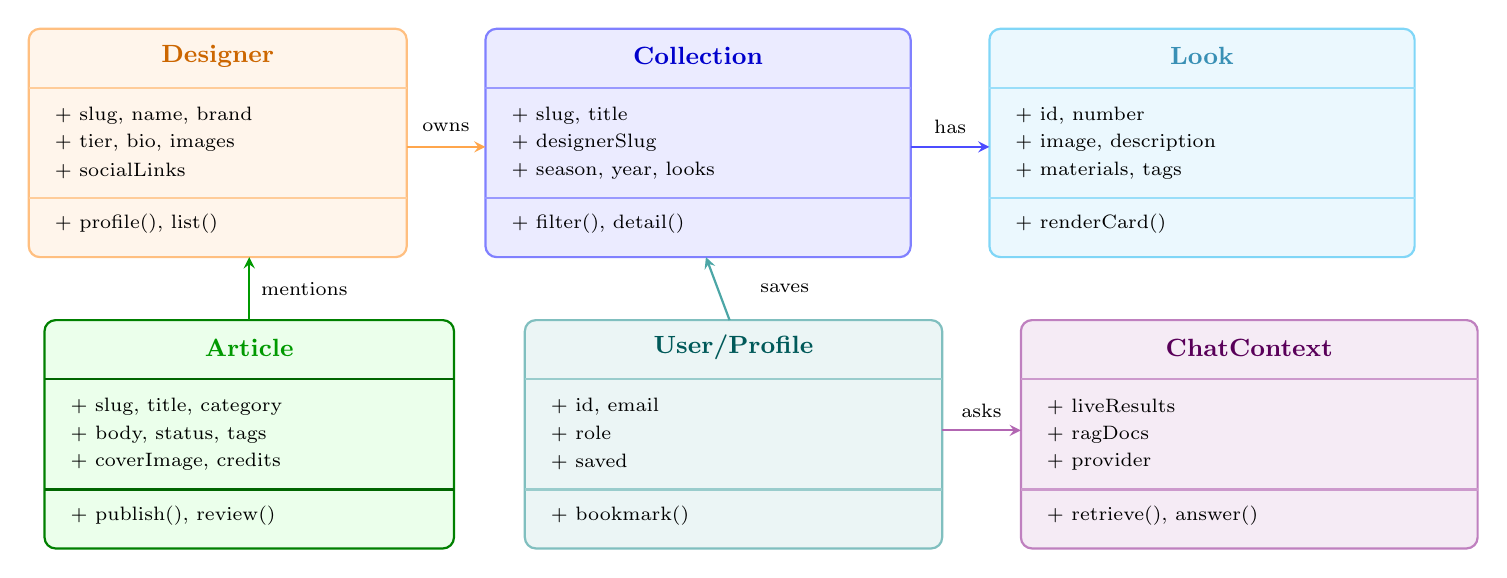
\begin{tikzpicture}[x=1cm,y=1cm,>=stealth,thick]
  % Designer
  \draw[rounded corners=4pt, fill=orange!8, draw=orange!50] (0,6.4) rectangle (4.8,9.3);
  \node[font=\small\bfseries, text=orange!80!black] at (2.4,8.95) {Designer};
  \draw[orange!40] (0,8.55) -- (4.8,8.55);
  \node[anchor=west,font=\scriptsize] at (0.2,8.20) {+ slug, name, brand};
  \node[anchor=west,font=\scriptsize] at (0.2,7.85) {+ tier, bio, images};
  \node[anchor=west,font=\scriptsize] at (0.2,7.50) {+ socialLinks};
  \draw[orange!40] (0,7.15) -- (4.8,7.15);
  \node[anchor=west,font=\scriptsize] at (0.2,6.82) {+ profile(), list()};

  % Collection
  \draw[rounded corners=4pt, fill=blue!8, draw=blue!50] (5.8,6.4) rectangle (11.2,9.3);
  \node[font=\small\bfseries, text=blue!80!black] at (8.5,8.95) {Collection};
  \draw[blue!40] (5.8,8.55) -- (11.2,8.55);
  \node[anchor=west,font=\scriptsize] at (6.0,8.20) {+ slug, title};
  \node[anchor=west,font=\scriptsize] at (6.0,7.85) {+ designerSlug};
  \node[anchor=west,font=\scriptsize] at (6.0,7.50) {+ season, year, looks};
  \draw[blue!40] (5.8,7.15) -- (11.2,7.15);
  \node[anchor=west,font=\scriptsize] at (6.0,6.82) {+ filter(), detail()};

  % Look
  \draw[rounded corners=4pt, fill=cyan!8, draw=cyan!50] (12.2,6.4) rectangle (17.6,9.3);
  \node[font=\small\bfseries, text=cyan!70!black] at (14.9,8.95) {Look};
  \draw[cyan!40] (12.2,8.55) -- (17.6,8.55);
  \node[anchor=west,font=\scriptsize] at (12.4,8.20) {+ id, number};
  \node[anchor=west,font=\scriptsize] at (12.4,7.85) {+ image, description};
  \node[anchor=west,font=\scriptsize] at (12.4,7.50) {+ materials, tags};
  \draw[cyan!40] (12.2,7.15) -- (17.6,7.15);
  \node[anchor=west,font=\scriptsize] at (12.4,6.82) {+ renderCard()};

  % Article
  \draw[rounded corners=4pt, fill=green!8, draw=green!50!black] (0.2,2.7) rectangle (5.4,5.6);
  \node[font=\small\bfseries, text=green!60!black] at (2.8,5.25) {Article};
  \draw[green!40!black] (0.2,4.85) -- (5.4,4.85);
  \node[anchor=west,font=\scriptsize] at (0.4,4.50) {+ slug, title, category};
  \node[anchor=west,font=\scriptsize] at (0.4,4.15) {+ body, status, tags};
  \node[anchor=west,font=\scriptsize] at (0.4,3.80) {+ coverImage, credits};
  \draw[green!40!black] (0.2,3.45) -- (5.4,3.45);
  \node[anchor=west,font=\scriptsize] at (0.4,3.12) {+ publish(), review()};

  % User/Profile
  \draw[rounded corners=4pt, fill=teal!8, draw=teal!50] (6.3,2.7) rectangle (11.6,5.6);
  \node[font=\small\bfseries, text=teal!70!black] at (8.95,5.25) {User/Profile};
  \draw[teal!40] (6.3,4.85) -- (11.6,4.85);
  \node[anchor=west,font=\scriptsize] at (6.5,4.50) {+ id, email};
  \node[anchor=west,font=\scriptsize] at (6.5,4.15) {+ role};
  \node[anchor=west,font=\scriptsize] at (6.5,3.80) {+ saved};
  \draw[teal!40] (6.3,3.45) -- (11.6,3.45);
  \node[anchor=west,font=\scriptsize] at (6.5,3.12) {+ bookmark()};

  % ChatContext
  \draw[rounded corners=4pt, fill=violet!8, draw=violet!50] (12.6,2.7) rectangle (18.4,5.6);
  \node[font=\small\bfseries, text=violet!70!black] at (15.5,5.25) {ChatContext};
  \draw[violet!40] (12.6,4.85) -- (18.4,4.85);
  \node[anchor=west,font=\scriptsize] at (12.8,4.50) {+ liveResults};
  \node[anchor=west,font=\scriptsize] at (12.8,4.15) {+ ragDocs};
  \node[anchor=west,font=\scriptsize] at (12.8,3.80) {+ provider};
  \draw[violet!40] (12.6,3.45) -- (18.4,3.45);
  \node[anchor=west,font=\scriptsize] at (12.8,3.12) {+ retrieve(), answer()};

  % Relationships
  \draw[->, orange!70] (4.8,7.8) -- (5.8,7.8);
  \node[font=\scriptsize, fill=white, inner sep=1pt] at (5.3,8.05) {owns};
  \draw[->, blue!70] (11.2,7.8) -- (12.2,7.8);
  \node[font=\scriptsize, fill=white, inner sep=1pt] at (11.7,8.05) {has};
  \draw[->, green!60!black] (2.8,5.6) -- (2.8,6.4);
  \node[font=\scriptsize, fill=white, inner sep=1pt] at (3.5,6.0) {mentions};
  \draw[->, teal!70] (8.9,5.6) -- (8.6,6.4);
  \node[font=\scriptsize, fill=white, inner sep=1pt] at (9.6,6.0) {saves};
  \draw[->, violet!60] (11.6,4.2) -- (12.6,4.2);
  \node[font=\scriptsize, fill=white, inner sep=1pt] at (12.1,4.45) {asks};
\end{tikzpicture}
}
  \caption[Шинжилгээний класс диаграмм]{Шинжилгээний класс диаграмм}
  \label{fig:ch2-analysis-class}
\end{figure}

Зураг \ref{fig:ch2-analysis-class}-т Designer, Collection, Look, Article, User/Profile, ChatContext хоорондын холбоог харуулав. Эдгээр class нь дараагийн бүлгийн өгөгдлийн сангийн зохиомжид document, table, service, repository хэлбэрээр нарийвчилна. Жишээлбэл, Article ойлголт нь CouchDB дахь article document болно, User/Profile нь Supabase profile болон auth user-тай холбогдоно, Collection дотор look object nested байдлаар хадгалагдана.

\section{Шинжилгээний дарааллын диаграмм}
Дарааллын диаграмм нь нэг үйлдэл системийн хэсгүүдээр ямар дарааллаар дамжихыг харуулна. Энэ хэсэгт платформын хамгийн чухал admin workflow болох ``Нийтлэл нэмэх'' үйлдлийг сонгов. Админ нийтлэл нэмэх үед UI, authentication layer, protected API, repository, database гэсэн хэсгүүд дараалан оролцоно.

\begin{figure}[htbp]
  \centering
  \resizebox{\textwidth}{!}{\begin{tikzpicture}[x=1cm,y=1cm,>=stealth,thick]
  \tikzstyle{box}=[draw, rounded corners=4pt, minimum width=2.45cm, minimum height=0.8cm,
    text width=2.2cm, align=center, font=\scriptsize]
  \tikzstyle{msg}=[font=\scriptsize, fill=white, inner sep=1pt, text width=3.0cm, align=center]

  \node[box, fill=red!10, draw=red!40] (admin) at (0,0) {Админ};
  \node[box, fill=orange!10, draw=orange!40] (ui) at (3.3,0) {Admin UI};
  \node[box, fill=yellow!12, draw=yellow!50!black] (auth) at (6.6,0) {Auth\\role check};
  \node[box, fill=blue!10, draw=blue!50] (api) at (9.9,0) {Admin API};
  \node[box, fill=green!10, draw=green!50!black] (repo) at (13.2,0) {Content\\Repository};
  \node[box, fill=teal!10, draw=teal!50] (db) at (16.5,0) {CouchDB};

  \foreach \x in {0,3.3,6.6,9.9,13.2,16.5} {
    \draw[dashed, black!30] (\x,-0.5) -- (\x,-8.7);
  }

  \draw[->, red!60] (0,-1.1) -- node[msg, above] {1. Нийтлэл нэмэх form нээх} (3.3,-1.1);
  \draw[->, orange!60] (3.3,-2.0) -- node[msg, above] {2. Session авах} (6.6,-2.0);
  \draw[<-, orange!60] (3.3,-2.9) -- node[msg, above] {3. admin/editor эрх OK} (6.6,-2.9);
  \draw[->, red!60] (0,-3.8) -- node[msg, above] {4. Гарчиг, body, зураг, category бөглөх} (3.3,-3.8);
  \draw[->, blue!60] (3.3,-4.7) -- node[msg, above] {5. POST /api/admin/content/articles} (9.9,-4.7);
  \draw[->, yellow!60!black] (9.9,-5.6) -- node[msg, above] {6. requireContentAdmin()} (6.6,-5.6);
  \draw[<-, blue!60] (9.9,-6.5) -- node[msg, above] {7. Эрх баталгаажсан} (6.6,-6.5);
  \draw[->, green!60!black] (9.9,-7.4) -- node[msg, above] {8. upsertArticle()} (13.2,-7.4);
  \draw[->, teal!70] (13.2,-8.1) -- node[msg, above] {9. Document хадгалах} (16.5,-8.1);
  \draw[<-, orange!60] (3.3,-8.7) -- node[msg, above] {10. id, rev, status} (16.5,-8.7);
\end{tikzpicture}
}
  \caption[Нийтлэл нэмэх үйлдлийн дарааллын диаграмм]{Нийтлэл нэмэх үйлдлийн дарааллын диаграмм}
  \label{fig:ch2-sequence-article-create}
\end{figure}

Зураг \ref{fig:ch2-sequence-article-create}-аас харахад admin UI шууд database руу бичихгүй. Эхлээд session болон role шалгагдаж, дараа нь \texttt{/api/admin/content/articles} endpoint хүсэлтийг хүлээн авч, \texttt{ContentRepository} class-ийн \texttt{upsertArticle()} method-оор CouchDB document хадгална. Энэ урсгал нь frontend, API, database-ийн хариуцлагыг шинжилгээний түвшинд ялгаж өгч байна.

\section{Үйл ажиллагааны диаграмм}
Үйл ажиллагааны диаграмм нь хэрэглэгчийн процессын эхлэл, шийдвэрийн цэг, төгсгөлийг харуулна. Энэ платформын public хэрэглэгчийн хамгийн нийтлэг процесс нь нийтлэл эсвэл collection хайж унших явдал юм. Хэрэглэгч нүүр эсвэл archive/editorial хуудас нээгээд, search эсвэл filter ашиглаж, тохирох контент олдвол detail page руу орж уншина. Үр дүн олдохгүй бол AI туслах эсвэл өөр query ашиглах боломжтой.

\begin{figure}[htbp]
  \centering
  \resizebox{0.52\textwidth}{!}{\begin{tikzpicture}[x=1cm,y=1cm,>=stealth,thick]
  \tikzstyle{action}=[draw, rounded corners=5pt, minimum width=3.8cm, minimum height=0.7cm,
    font=\scriptsize, align=center]
  \tikzstyle{decision}=[diamond, draw, aspect=2.2, font=\scriptsize, align=center, inner sep=1pt]

  \node[circle, draw, minimum size=0.5cm, fill=black] (start) at (0,0) {};
  \node[action, fill=blue!10, draw=blue!50] (open) at (0,-1.0) {Сайт нээх};
  \node[action, fill=blue!10, draw=blue!50] (catalog) at (0,-2.1) {Archive / Editorial үзэх};
  \node[action, fill=cyan!10, draw=cyan!50] (searchfilter) at (0,-3.2) {Search эсвэл filter хийх};
  \node[decision, fill=yellow!15, draw=yellow!60!black] (found) at (0,-4.5) {Content олдсон уу?};
  \node[action, fill=violet!10, draw=violet!50] (ai) at (-4.4,-5.7) {AI туслахаас асуух};
  \node[action, fill=green!10, draw=green!50!black] (detail) at (0,-6.7) {Collection / Article нээх};
  \node[action, fill=green!10, draw=green!50!black] (view) at (0,-7.8) {Look, material, designer үзэх};
  \node[decision, fill=yellow!15, draw=yellow!60!black] (save) at (0,-9.1) {Хадгалах уу?};
  \node[action, fill=teal!10, draw=teal!50] (login) at (4.6,-10.2) {Login / Bookmark};
  \node[action, fill=blue!10, draw=blue!50] (next) at (0,-11.1) {Дараагийн content үзэх};
  \node[circle, draw=black, line width=1.5pt, minimum size=0.5cm, fill=black] (end) at (0,-12.2) {};
  \node[circle, draw=black, minimum size=0.75cm] at (0,-12.2) {};

  \draw[->, blue!70] (start) -- (open);
  \draw[->, blue!70] (open) -- (catalog);
  \draw[->, cyan!70] (catalog) -- (searchfilter);
  \draw[->, black!60] (searchfilter) -- (found);
  \draw[->, red!60] (found) -- node[above, font=\scriptsize, text=red!70!black] {Үгүй} (ai);
  \draw[->, violet!60] (ai.south) |- (detail.west);
  \draw[->, green!60!black] (found) -- node[right, font=\scriptsize, text=green!60!black] {Тийм} (detail);
  \draw[->, green!60!black] (detail) -- (view);
  \draw[->, black!60] (view) -- (save);
  \draw[->, teal!70] (save) -- node[above, font=\scriptsize, text=teal!70!black] {Тийм} (login);
  \draw[->, teal!60] (login.south) |- (next.east);
  \draw[->, black!60] (save) -- node[left, font=\scriptsize] {Үгүй} (next);
  \draw[->, black!60] (next) -- (end);
\end{tikzpicture}
}
  \caption[Хэрэглэгч нийтлэл хайж унших үйл ажиллагааны диаграмм]{Хэрэглэгч нийтлэл хайж унших үйл ажиллагааны диаграмм}
  \label{fig:ch2-activity-search-read}
\end{figure}

Зураг \ref{fig:ch2-activity-search-read}-т ``Content олдсон уу?'' гэсэн шийдвэрийн цэг байна. Хэрэв үр дүн олдвол collection эсвэл article detail нээгдэнэ. Үр дүн олдохгүй бол хэрэглэгч AI туслахаас асуух эсвэл дахин хайх боломжтой. Энэ нь хэрэглэгчийн туршлагыг таслахгүй, empty state-ийг зөв зохион байгуулах шаардлагатайг харуулна.

\section{Өгөгдлийн шаардлага ба контентын бүтэц}
Платформд хэрэглэгчийн өгөгдөл, админ хэрэглэгчийн эрхийн өгөгдөл, нийтлэлийн өгөгдөл, category, tag, зураг, collection, archive, authentication data, \texttt{created\_at}, \texttt{updated\_at}, slug, thumbnail, content body зэрэг олон төрлийн өгөгдөл шаардлагатай. Fashion magazine platform учраас өгөгдөл нь зөвхөн текст бус, зурагт content, designer relation, collection metadata, look image, material, season зэрэг шинжийг хамарна.

\begin{longtable}{|L{0.18\textwidth}|L{0.38\textwidth}|L{0.30\textwidth}|}
  \hline
  \textbf{Өгөгдөл} & \textbf{Тайлбар} & \textbf{Ашиглагдах хэсэг} \\ \hline
  User/Profile & id, email, name, role, avatar, bookmark холбоо & Login, profile, admin authorization \\ \hline
  Article & id, slug, title, subtitle, description, body, thumbnail, images, category, tags, author, published date, status & Editorial, article detail, archive, search, admin CMS \\ \hline
  Category & Контентыг fashion, beauty, lifestyle, trend зэрэг бүлэгт ангилах & Navigation, filter, admin form \\ \hline
  Tag & Нарийвчилсан хайлт, related content, trend grouping хийх түлхүүр үг & Search, related content, article detail \\ \hline
  Image/Asset & Cover, thumbnail, look, designer profile image хадгалах & Article, collection, lookbook, designer profile \\ \hline
  Designer & slug, name, brand, bio, tier, social link, profile image & Designer directory, collection relation \\ \hline
  Collection & slug, title, designer, season, year, looks, materials, tags & Archive, collection detail, search \\ \hline
  Archive & Өмнөх collection, нийтлэл, designer, season/year metadata-ийн нэгтгэл & Archive page, AI context, search \\ \hline
  Auth data & session, token/cookie, role, access control state & Login, protected admin route, API authorization \\ \hline
  RAG document & title, content, category, tags, source, brand/content slug & AI chatbot context \\ \hline
  \caption{Өгөгдлийн шаардлага}
  \label{tab:data-requirements-ch2}\\
\end{longtable}

Контентын бүтэц нь Fashion news, Trend, Collection, Interview, Editorial, Lookbook, Brand story, Archive гэсэн бүлгүүдтэй байж болно. Энэ бүтэц нь user-facing navigation болон admin-facing metadata хоёрт зэрэг ашиглагдана.

\section{Бизнес процессын шинжилгээ}
Платформын бизнес процесс нь контент бэлтгэх, системд бүртгэх, шалгах, нийтлэх, хэрэглэгчид хүргэх, хэрэглэгчийн хайлт/ангиллаар дахин олгох гэсэн дараалалтай. Гол процессууд нь контент нийтлэх процесс, хэрэглэгч контент үзэх процесс, админ контент удирдах процесс, хайлт/ангиллаар контент олох процесс юм.

\begin{longtable}{|L{0.18\textwidth}|L{0.16\textwidth}|L{0.32\textwidth}|L{0.16\textwidth}|}
  \hline
  \textbf{Процесс} & \textbf{Оролцогч} & \textbf{Үндсэн алхам} & \textbf{Гарах үр дүн} \\ \hline
  Контент нийтлэх & Редактор, админ & Админ нэвтэрнэ; нийтлэлийн агуулга бэлтгэнэ; зураг оруулна; category/tag сонгоно; draft/review/published төлөвөөр хадгална & Нийтлэл хэрэглэгчийн хэсэгт харагдана \\ \hline
  Контент үзэх & Зочин, хэрэглэгч & Нүүр, editorial, archive, designer page нээнэ; нийтлэл эсвэл collection сонгоно & Хэрэглэгч загварын мэдээлэл уншина \\ \hline
  Контент удирдах & Админ, редактор & Article, collection, designer, asset жагсаалт харна; нэмнэ, засна, устгана & Контентын сан шинэчлэгдэнэ \\ \hline
  Хайлт ба ангилал & Зочин, хэрэглэгч & Search query бичнэ; category/filter сонгоно; үр дүнгээс detail нээнэ & Хэрэглэгч хэрэгтэй контентоо хурдан олно \\ \hline
  Эрх удирдах & Админ & Invite илгээнэ; user role өөрчилнө; editor/admin эрх шалгана & CMS хэрэглэгчийн эрх зохицуулагдана \\ \hline
  AI лавлагаа & Бүртгэлтэй хэрэглэгч & Chat асуулт илгээнэ; live/RAG context хайна; хариу буцаана & Архивт тулгуурласан лавлагаа өгнө \\ \hline
  \caption{Контент нийтлэх ба удирдах бизнес процесс}
  \label{tab:business-process-ch2}\\
\end{longtable}

Эдгээр процессын сайжруулах боломж нь workflow-д audit log, notification, advanced search, automatic RAG sync, image CDN зэрэг нэмэлтүүд оруулах явдал юм. Гэвч дипломын үндсэн хүрээнд content management, public display, search, authentication, authorization-ийг MVP түвшинд хэрэгжүүлэхэд төвлөрнө.

\section*{Бүлгийн дүгнэлт}
\addcontentsline{toc}{section}{Бүлгийн дүгнэлт}

Хоёрдугаар бүлгээр Монголын загварын контент одоогоор олон эх сурвалжид тархсан, нэгдсэн fashion magazine болон digital archive бүтэц хомс байгаа асуудлыг тодорхойлов. Үүнээс Anoce/MFA платформ хөгжүүлэх хэрэгцээ гарч, хэрэглэгчийн төрөл, функциональ болон функциональ бус шаардлага, use case, class, sequence, activity diagram, өгөгдлийн шаардлага, бизнес процессын шинжилгээ боловсруулагдлаа. Энэхүү шинжилгээнд үндэслэн гуравдугаар бүлэгт платформын архитектур, API, өгөгдлийн сан, UI/UX зохиомж, admin болон security шийдлийг нарийвчлан боловсруулна.
